\section{Adjusting the Parameters}
\label{sec:add.parameters}

Making the archetypal model continuous is in direct conflict with varying the parameters $\alpha = g_R\left(\frac{1}{4}\right)$ and $\beta = c_L$ individually.
But we can make the archetypal model always increasing.

The fixed parameters in the archetypal are $a_L = 4, b_L = -\frac{1}{2},$ and $g_R\left(\frac{1}{4}\right)$.
We can see in \Cref{fig:add.arch} that only the branches $f_\A$ and $f_\C$ are not monotonously increasing.
Of the three fixed parameters, $a_L$ and $b_L$ influence the shape of the branches $f_\A$ and $f_\C$.
We adjust these parameters to make the branches monotonously increasing.
The new parameter values are $a_L = 1$ and $b_L = \frac{1}{2}$.
The new shape of the function can be seen in \Cref{fig:add.arch.new}, now all branches are monotonously increasing.

\begin{figure}
	\centering
	\subfloat[Function shape]{
		\todo{Add pic of the new model fct}
		\label{fig:add.arch.new}
	}\\
	\subfloat[2D scan of periods]{
		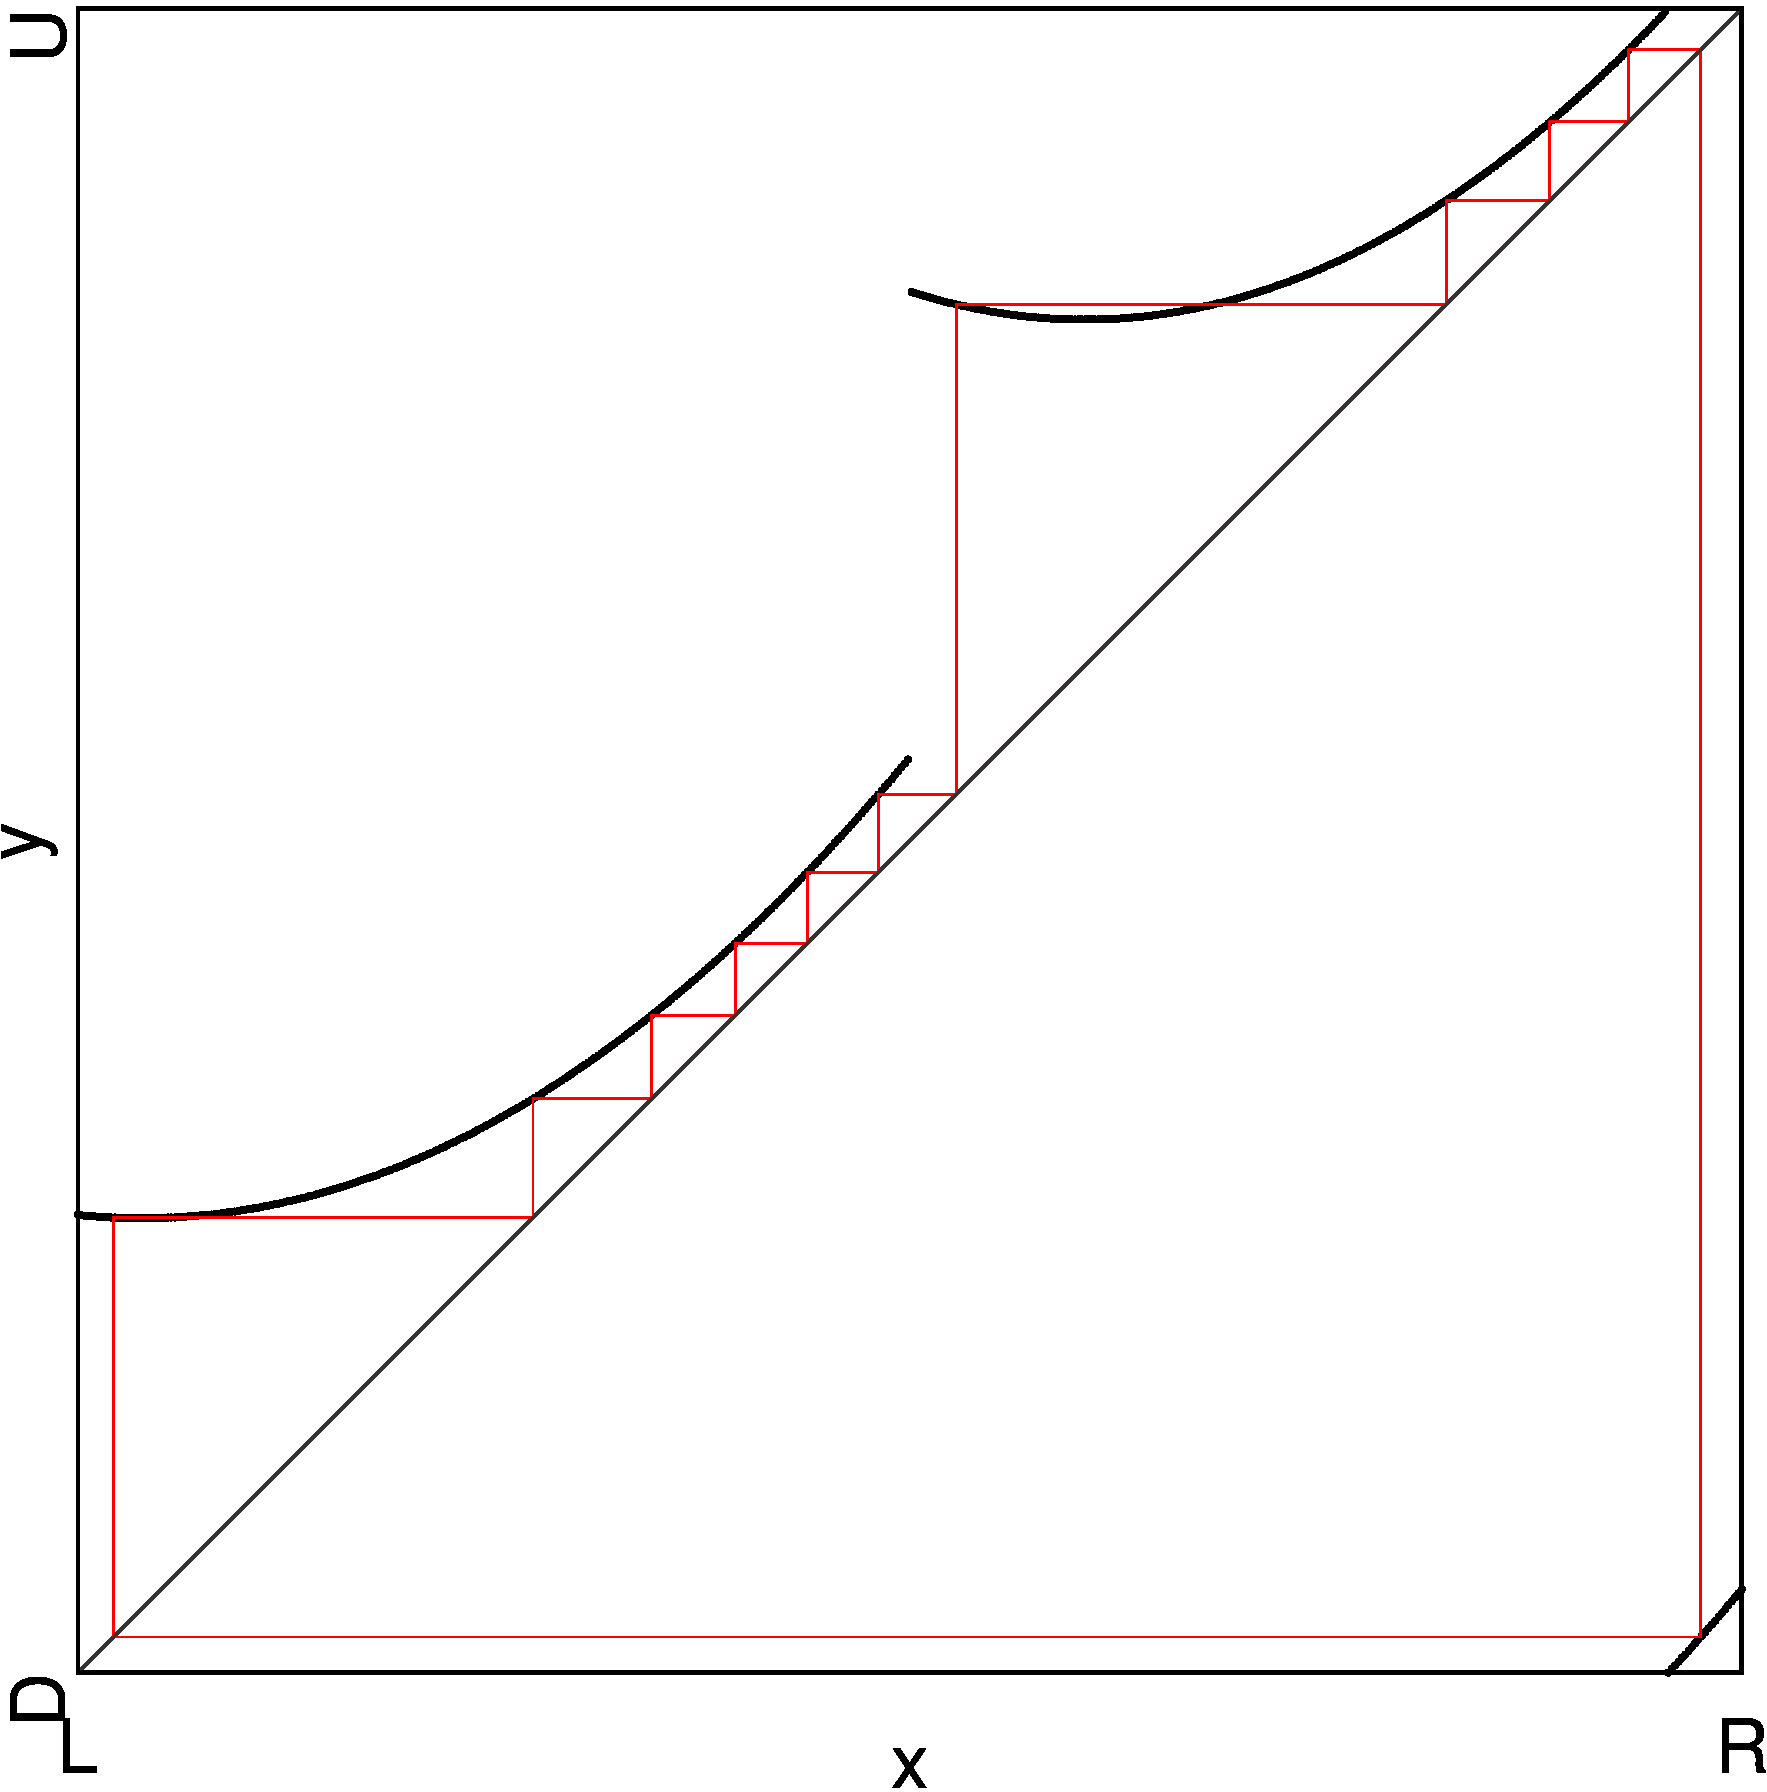
\includegraphics[width=.4 \textwidth]{62_MinimalRepr_Adding/2D_Period_1/result.png}
		\label{fig:add.arch.new.period}
	}
	\caption[Model function shape and 2D period scan of the increasing archetypal model]{
		Model function shape and 2D period scan of the increasing archetypal model.
		\todo{Expand on caption}
	}
\end{figure}

\Cref{fig:add.arch.new.period} shows a 2D scan of the periods in the archetypal model with the new parameters.
We will refer to this model as the increasing archetypal model.
In this scan, we can see that the ``type B'' parameter regions disappeared and ``type A'' parameter regions of the same chain seem to start overlapping.
Also, in between the chains there are now small parameter regions with much higher periods.
This looks like period adding and, we will explore it in the following sections.
But first, we will take a closer look at how the bifurcations structures change when adjusting the parameters $a_L$ and $b_L$ to make the branches $f_\A$ and $f_\C$ increasing.
